\documentclass{standalone}
\usepackage{tikz}
\usepackage{xcolor}
\usetikzlibrary{patterns, positioning}

    \usetikzlibrary{calc}
    \usepackage{relsize}
    \tikzset{fontscale/.style = {font=\relsize{#1}}}
\begin{document}
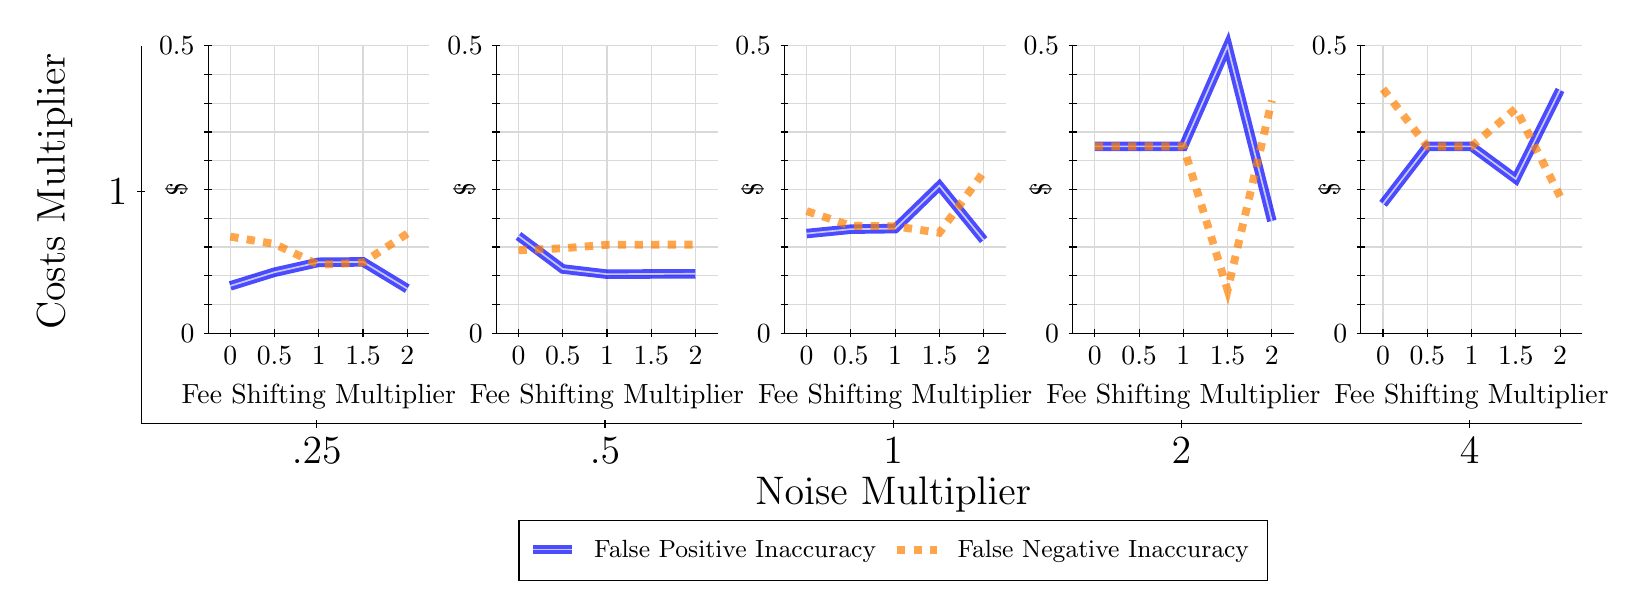
\begin{tikzpicture}
\draw[black] (1.7,1.5) -- (1.7,6.3);
\node[rotate=90, fontscale=2, anchor=center] at (0.6, 4.45) {Costs Multiplier};
\draw[black] (1.65,4.45) -- (1.75,4.45);
\node[fontscale=2, anchor=east] at (1.65, 4.45) {1};

\draw[black] (1.7,1.5) -- (20,1.5);
\node[fontscale=2, anchor=center] at (11.25, 0.6) {Noise Multiplier};
\draw[black] (3.93,1.45) -- (3.93,1.55);
\node[fontscale=2, anchor=north] at (3.93, 1.45) {.25};
\draw[black] (7.59,1.45) -- (7.59,1.55);
\node[fontscale=2, anchor=north] at (7.59, 1.45) {.5};
\draw[black] (11.25,1.45) -- (11.25,1.55);
\node[fontscale=2, anchor=north] at (11.25, 1.45) {1};
\draw[black] (14.91,1.45) -- (14.91,1.55);
\node[fontscale=2, anchor=north] at (14.91, 1.45) {2};
\draw[black] (18.57,1.45) -- (18.57,1.55);
\node[fontscale=2, anchor=north] at (18.57, 1.45) {4};


\draw[gray!30] (2.55,2.65) -- (5.36,2.65);
\draw[gray!30] (2.55,3.015) -- (5.36,3.015);
\draw[gray!30] (2.55,3.38) -- (5.36,3.38);
\draw[gray!30] (2.55,3.745) -- (5.36,3.745);
\draw[gray!30] (2.55,4.11) -- (5.36,4.11);
\draw[gray!30] (2.55,4.475) -- (5.36,4.475);
\draw[gray!30] (2.55,4.84) -- (5.36,4.84);
\draw[gray!30] (2.55,5.205) -- (5.36,5.205);
\draw[gray!30] (2.55,5.57) -- (5.36,5.57);
\draw[gray!30] (2.55,5.935) -- (5.36,5.935);
\draw[gray!30] (2.55,6.3) -- (5.36,6.3);
\draw[gray!30] (2.831,2.65) -- (2.831,6.3);
\draw[gray!30] (3.393,2.65) -- (3.393,6.3);
\draw[gray!30] (3.955,2.65) -- (3.955,6.3);
\draw[gray!30] (4.517,2.65) -- (4.517,6.3);
\draw[gray!30] (5.079,2.65) -- (5.079,6.3);
\draw[black] (2.55,2.65) -- (2.55,6.3);
\node[rotate=90, fontscale=0.7, anchor=center] at (2.15, 4.475) {\$};
\draw[black] (2.5,2.65) -- (2.6,2.65);
\node[fontscale=0.7, anchor=east] at (2.5, 2.65) {0};
\draw[black] (2.5,3.015) -- (2.6,3.015);
\node[fontscale=0.7, anchor=east] at (2.5, 3.015) { };
\draw[black] (2.5,3.38) -- (2.6,3.38);
\node[fontscale=0.7, anchor=east] at (2.5, 3.38) { };
\draw[black] (2.5,3.745) -- (2.6,3.745);
\node[fontscale=0.7, anchor=east] at (2.5, 3.745) { };
\draw[black] (2.5,4.11) -- (2.6,4.11);
\node[fontscale=0.7, anchor=east] at (2.5, 4.11) { };
\draw[black] (2.5,4.475) -- (2.6,4.475);
\node[fontscale=0.7, anchor=east] at (2.5, 4.475) { };
\draw[black] (2.5,4.84) -- (2.6,4.84);
\node[fontscale=0.7, anchor=east] at (2.5, 4.84) { };
\draw[black] (2.5,5.205) -- (2.6,5.205);
\node[fontscale=0.7, anchor=east] at (2.5, 5.205) { };
\draw[black] (2.5,5.57) -- (2.6,5.57);
\node[fontscale=0.7, anchor=east] at (2.5, 5.57) { };
\draw[black] (2.5,5.935) -- (2.6,5.935);
\node[fontscale=0.7, anchor=east] at (2.5, 5.935) { };
\draw[black] (2.5,6.3) -- (2.6,6.3);
\node[fontscale=0.7, anchor=east] at (2.5, 6.3) {0.5};

\draw[black] (2.55,2.65) -- (5.36,2.65);
\node[fontscale=0.7, anchor=center] at (3.955, 1.85) {Fee Shifting Multiplier};
\draw[black] (2.831,2.6) -- (2.831,2.7);
\node[fontscale=0.7, anchor=north] at (2.831, 2.6) {0};
\draw[black] (3.393,2.6) -- (3.393,2.7);
\node[fontscale=0.7, anchor=north] at (3.393, 2.6) {0.5};
\draw[black] (3.955,2.6) -- (3.955,2.7);
\node[fontscale=0.7, anchor=north] at (3.955, 2.6) {1};
\draw[black] (4.517,2.6) -- (4.517,2.7);
\node[fontscale=0.7, anchor=north] at (4.517, 2.6) {1.5};
\draw[black] (5.079,2.6) -- (5.079,2.7);
\node[fontscale=0.7, anchor=north] at (5.079, 2.6) {2};

\draw[blue, opacity=0.70, line width=0.5mm, double] (2.831,3.2508) -- (3.393,3.4246) -- (3.955,3.5509) -- (4.517,3.5556) -- (5.079,3.2149);
\draw[orange, opacity=0.70, line width=1mm, dashed] (2.831,3.8768) -- (3.393,3.7833) -- (3.955,3.5183) -- (4.517,3.5478) -- (5.079,3.9147);

\draw[gray!30] (6.21,2.65) -- (9.02,2.65);
\draw[gray!30] (6.21,3.015) -- (9.02,3.015);
\draw[gray!30] (6.21,3.38) -- (9.02,3.38);
\draw[gray!30] (6.21,3.745) -- (9.02,3.745);
\draw[gray!30] (6.21,4.11) -- (9.02,4.11);
\draw[gray!30] (6.21,4.475) -- (9.02,4.475);
\draw[gray!30] (6.21,4.84) -- (9.02,4.84);
\draw[gray!30] (6.21,5.205) -- (9.02,5.205);
\draw[gray!30] (6.21,5.57) -- (9.02,5.57);
\draw[gray!30] (6.21,5.935) -- (9.02,5.935);
\draw[gray!30] (6.21,6.3) -- (9.02,6.3);
\draw[gray!30] (6.491,2.65) -- (6.491,6.3);
\draw[gray!30] (7.053,2.65) -- (7.053,6.3);
\draw[gray!30] (7.615,2.65) -- (7.615,6.3);
\draw[gray!30] (8.177,2.65) -- (8.177,6.3);
\draw[gray!30] (8.739,2.65) -- (8.739,6.3);
\draw[black] (6.21,2.65) -- (6.21,6.3);
\node[rotate=90, fontscale=0.7, anchor=center] at (5.81, 4.475) {\$};
\draw[black] (6.16,2.65) -- (6.26,2.65);
\node[fontscale=0.7, anchor=east] at (6.16, 2.65) {0};
\draw[black] (6.16,3.015) -- (6.26,3.015);
\node[fontscale=0.7, anchor=east] at (6.16, 3.015) { };
\draw[black] (6.16,3.38) -- (6.26,3.38);
\node[fontscale=0.7, anchor=east] at (6.16, 3.38) { };
\draw[black] (6.16,3.745) -- (6.26,3.745);
\node[fontscale=0.7, anchor=east] at (6.16, 3.745) { };
\draw[black] (6.16,4.11) -- (6.26,4.11);
\node[fontscale=0.7, anchor=east] at (6.16, 4.11) { };
\draw[black] (6.16,4.475) -- (6.26,4.475);
\node[fontscale=0.7, anchor=east] at (6.16, 4.475) { };
\draw[black] (6.16,4.84) -- (6.26,4.84);
\node[fontscale=0.7, anchor=east] at (6.16, 4.84) { };
\draw[black] (6.16,5.205) -- (6.26,5.205);
\node[fontscale=0.7, anchor=east] at (6.16, 5.205) { };
\draw[black] (6.16,5.57) -- (6.26,5.57);
\node[fontscale=0.7, anchor=east] at (6.16, 5.57) { };
\draw[black] (6.16,5.935) -- (6.26,5.935);
\node[fontscale=0.7, anchor=east] at (6.16, 5.935) { };
\draw[black] (6.16,6.3) -- (6.26,6.3);
\node[fontscale=0.7, anchor=east] at (6.16, 6.3) {0.5};

\draw[black] (6.21,2.65) -- (9.02,2.65);
\node[fontscale=0.7, anchor=center] at (7.615, 1.85) {Fee Shifting Multiplier};
\draw[black] (6.491,2.6) -- (6.491,2.7);
\node[fontscale=0.7, anchor=north] at (6.491, 2.6) {0};
\draw[black] (7.053,2.6) -- (7.053,2.7);
\node[fontscale=0.7, anchor=north] at (7.053, 2.6) {0.5};
\draw[black] (7.615,2.6) -- (7.615,2.7);
\node[fontscale=0.7, anchor=north] at (7.615, 2.6) {1};
\draw[black] (8.177,2.6) -- (8.177,2.7);
\node[fontscale=0.7, anchor=north] at (8.177, 2.6) {1.5};
\draw[black] (8.739,2.6) -- (8.739,2.7);
\node[fontscale=0.7, anchor=north] at (8.739, 2.6) {2};

\draw[blue, opacity=0.70, line width=0.5mm, double] (6.491,3.8857) -- (7.053,3.4659) -- (7.615,3.3997) -- (8.177,3.4023) -- (8.739,3.4048);
\draw[orange, opacity=0.70, line width=1mm, dashed] (6.491,3.7034) -- (7.053,3.7286) -- (7.615,3.7729) -- (8.177,3.7741) -- (8.739,3.7753);

\draw[gray!30] (9.87,2.65) -- (12.68,2.65);
\draw[gray!30] (9.87,3.015) -- (12.68,3.015);
\draw[gray!30] (9.87,3.38) -- (12.68,3.38);
\draw[gray!30] (9.87,3.745) -- (12.68,3.745);
\draw[gray!30] (9.87,4.11) -- (12.68,4.11);
\draw[gray!30] (9.87,4.475) -- (12.68,4.475);
\draw[gray!30] (9.87,4.84) -- (12.68,4.84);
\draw[gray!30] (9.87,5.205) -- (12.68,5.205);
\draw[gray!30] (9.87,5.57) -- (12.68,5.57);
\draw[gray!30] (9.87,5.935) -- (12.68,5.935);
\draw[gray!30] (9.87,6.3) -- (12.68,6.3);
\draw[gray!30] (10.151,2.65) -- (10.151,6.3);
\draw[gray!30] (10.713,2.65) -- (10.713,6.3);
\draw[gray!30] (11.275,2.65) -- (11.275,6.3);
\draw[gray!30] (11.837,2.65) -- (11.837,6.3);
\draw[gray!30] (12.399,2.65) -- (12.399,6.3);
\draw[black] (9.87,2.65) -- (9.87,6.3);
\node[rotate=90, fontscale=0.7, anchor=center] at (9.47, 4.475) {\$};
\draw[black] (9.82,2.65) -- (9.92,2.65);
\node[fontscale=0.7, anchor=east] at (9.82, 2.65) {0};
\draw[black] (9.82,3.015) -- (9.92,3.015);
\node[fontscale=0.7, anchor=east] at (9.82, 3.015) { };
\draw[black] (9.82,3.38) -- (9.92,3.38);
\node[fontscale=0.7, anchor=east] at (9.82, 3.38) { };
\draw[black] (9.82,3.745) -- (9.92,3.745);
\node[fontscale=0.7, anchor=east] at (9.82, 3.745) { };
\draw[black] (9.82,4.11) -- (9.92,4.11);
\node[fontscale=0.7, anchor=east] at (9.82, 4.11) { };
\draw[black] (9.82,4.475) -- (9.92,4.475);
\node[fontscale=0.7, anchor=east] at (9.82, 4.475) { };
\draw[black] (9.82,4.84) -- (9.92,4.84);
\node[fontscale=0.7, anchor=east] at (9.82, 4.84) { };
\draw[black] (9.82,5.205) -- (9.92,5.205);
\node[fontscale=0.7, anchor=east] at (9.82, 5.205) { };
\draw[black] (9.82,5.57) -- (9.92,5.57);
\node[fontscale=0.7, anchor=east] at (9.82, 5.57) { };
\draw[black] (9.82,5.935) -- (9.92,5.935);
\node[fontscale=0.7, anchor=east] at (9.82, 5.935) { };
\draw[black] (9.82,6.3) -- (9.92,6.3);
\node[fontscale=0.7, anchor=east] at (9.82, 6.3) {0.5};

\draw[black] (9.87,2.65) -- (12.68,2.65);
\node[fontscale=0.7, anchor=center] at (11.275, 1.85) {Fee Shifting Multiplier};
\draw[black] (10.151,2.6) -- (10.151,2.7);
\node[fontscale=0.7, anchor=north] at (10.151, 2.6) {0};
\draw[black] (10.713,2.6) -- (10.713,2.7);
\node[fontscale=0.7, anchor=north] at (10.713, 2.6) {0.5};
\draw[black] (11.275,2.6) -- (11.275,2.7);
\node[fontscale=0.7, anchor=north] at (11.275, 2.6) {1};
\draw[black] (11.837,2.6) -- (11.837,2.7);
\node[fontscale=0.7, anchor=north] at (11.837, 2.6) {1.5};
\draw[black] (12.399,2.6) -- (12.399,2.7);
\node[fontscale=0.7, anchor=north] at (12.399, 2.6) {2};

\draw[blue, opacity=0.70, line width=0.5mm, double] (10.151,3.9154) -- (10.713,3.9714) -- (11.275,3.9786) -- (11.837,4.5249) -- (12.399,3.833);
\draw[orange, opacity=0.70, line width=1mm, dashed] (10.151,4.2009) -- (10.713,4.0144) -- (11.275,4.0083) -- (11.837,3.9252) -- (12.399,4.6956);

\draw[gray!30] (13.53,2.65) -- (16.34,2.65);
\draw[gray!30] (13.53,3.015) -- (16.34,3.015);
\draw[gray!30] (13.53,3.38) -- (16.34,3.38);
\draw[gray!30] (13.53,3.745) -- (16.34,3.745);
\draw[gray!30] (13.53,4.11) -- (16.34,4.11);
\draw[gray!30] (13.53,4.475) -- (16.34,4.475);
\draw[gray!30] (13.53,4.84) -- (16.34,4.84);
\draw[gray!30] (13.53,5.205) -- (16.34,5.205);
\draw[gray!30] (13.53,5.57) -- (16.34,5.57);
\draw[gray!30] (13.53,5.935) -- (16.34,5.935);
\draw[gray!30] (13.53,6.3) -- (16.34,6.3);
\draw[gray!30] (13.811,2.65) -- (13.811,6.3);
\draw[gray!30] (14.373,2.65) -- (14.373,6.3);
\draw[gray!30] (14.935,2.65) -- (14.935,6.3);
\draw[gray!30] (15.497,2.65) -- (15.497,6.3);
\draw[gray!30] (16.059,2.65) -- (16.059,6.3);
\draw[black] (13.53,2.65) -- (13.53,6.3);
\node[rotate=90, fontscale=0.7, anchor=center] at (13.13, 4.475) {\$};
\draw[black] (13.48,2.65) -- (13.58,2.65);
\node[fontscale=0.7, anchor=east] at (13.48, 2.65) {0};
\draw[black] (13.48,3.015) -- (13.58,3.015);
\node[fontscale=0.7, anchor=east] at (13.48, 3.015) { };
\draw[black] (13.48,3.38) -- (13.58,3.38);
\node[fontscale=0.7, anchor=east] at (13.48, 3.38) { };
\draw[black] (13.48,3.745) -- (13.58,3.745);
\node[fontscale=0.7, anchor=east] at (13.48, 3.745) { };
\draw[black] (13.48,4.11) -- (13.58,4.11);
\node[fontscale=0.7, anchor=east] at (13.48, 4.11) { };
\draw[black] (13.48,4.475) -- (13.58,4.475);
\node[fontscale=0.7, anchor=east] at (13.48, 4.475) { };
\draw[black] (13.48,4.84) -- (13.58,4.84);
\node[fontscale=0.7, anchor=east] at (13.48, 4.84) { };
\draw[black] (13.48,5.205) -- (13.58,5.205);
\node[fontscale=0.7, anchor=east] at (13.48, 5.205) { };
\draw[black] (13.48,5.57) -- (13.58,5.57);
\node[fontscale=0.7, anchor=east] at (13.48, 5.57) { };
\draw[black] (13.48,5.935) -- (13.58,5.935);
\node[fontscale=0.7, anchor=east] at (13.48, 5.935) { };
\draw[black] (13.48,6.3) -- (13.58,6.3);
\node[fontscale=0.7, anchor=east] at (13.48, 6.3) {0.5};

\draw[black] (13.53,2.65) -- (16.34,2.65);
\node[fontscale=0.7, anchor=center] at (14.935, 1.85) {Fee Shifting Multiplier};
\draw[black] (13.811,2.6) -- (13.811,2.7);
\node[fontscale=0.7, anchor=north] at (13.811, 2.6) {0};
\draw[black] (14.373,2.6) -- (14.373,2.7);
\node[fontscale=0.7, anchor=north] at (14.373, 2.6) {0.5};
\draw[black] (14.935,2.6) -- (14.935,2.7);
\node[fontscale=0.7, anchor=north] at (14.935, 2.6) {1};
\draw[black] (15.497,2.6) -- (15.497,2.7);
\node[fontscale=0.7, anchor=north] at (15.497, 2.6) {1.5};
\draw[black] (16.059,2.6) -- (16.059,2.7);
\node[fontscale=0.7, anchor=north] at (16.059, 2.6) {2};

\draw[blue, opacity=0.70, line width=0.5mm, double] (13.811,5.0225) -- (14.373,5.0225) -- (14.935,5.0225) -- (15.497,6.3) -- (16.059,4.0748);
\draw[orange, opacity=0.70, line width=1mm, dashed] (13.811,5.0225) -- (14.373,5.0225) -- (14.935,5.0225) -- (15.497,3.1975) -- (16.059,5.6054);

\draw[gray!30] (17.19,2.65) -- (20,2.65);
\draw[gray!30] (17.19,3.015) -- (20,3.015);
\draw[gray!30] (17.19,3.38) -- (20,3.38);
\draw[gray!30] (17.19,3.745) -- (20,3.745);
\draw[gray!30] (17.19,4.11) -- (20,4.11);
\draw[gray!30] (17.19,4.475) -- (20,4.475);
\draw[gray!30] (17.19,4.84) -- (20,4.84);
\draw[gray!30] (17.19,5.205) -- (20,5.205);
\draw[gray!30] (17.19,5.57) -- (20,5.57);
\draw[gray!30] (17.19,5.935) -- (20,5.935);
\draw[gray!30] (17.19,6.3) -- (20,6.3);
\draw[gray!30] (17.471,2.65) -- (17.471,6.3);
\draw[gray!30] (18.033,2.65) -- (18.033,6.3);
\draw[gray!30] (18.595,2.65) -- (18.595,6.3);
\draw[gray!30] (19.157,2.65) -- (19.157,6.3);
\draw[gray!30] (19.719,2.65) -- (19.719,6.3);
\draw[black] (17.19,2.65) -- (17.19,6.3);
\node[rotate=90, fontscale=0.7, anchor=center] at (16.79, 4.475) {\$};
\draw[black] (17.14,2.65) -- (17.24,2.65);
\node[fontscale=0.7, anchor=east] at (17.14, 2.65) {0};
\draw[black] (17.14,3.015) -- (17.24,3.015);
\node[fontscale=0.7, anchor=east] at (17.14, 3.015) { };
\draw[black] (17.14,3.38) -- (17.24,3.38);
\node[fontscale=0.7, anchor=east] at (17.14, 3.38) { };
\draw[black] (17.14,3.745) -- (17.24,3.745);
\node[fontscale=0.7, anchor=east] at (17.14, 3.745) { };
\draw[black] (17.14,4.11) -- (17.24,4.11);
\node[fontscale=0.7, anchor=east] at (17.14, 4.11) { };
\draw[black] (17.14,4.475) -- (17.24,4.475);
\node[fontscale=0.7, anchor=east] at (17.14, 4.475) { };
\draw[black] (17.14,4.84) -- (17.24,4.84);
\node[fontscale=0.7, anchor=east] at (17.14, 4.84) { };
\draw[black] (17.14,5.205) -- (17.24,5.205);
\node[fontscale=0.7, anchor=east] at (17.14, 5.205) { };
\draw[black] (17.14,5.57) -- (17.24,5.57);
\node[fontscale=0.7, anchor=east] at (17.14, 5.57) { };
\draw[black] (17.14,5.935) -- (17.24,5.935);
\node[fontscale=0.7, anchor=east] at (17.14, 5.935) { };
\draw[black] (17.14,6.3) -- (17.24,6.3);
\node[fontscale=0.7, anchor=east] at (17.14, 6.3) {0.5};

\draw[black] (17.19,2.65) -- (20,2.65);
\node[fontscale=0.7, anchor=center] at (18.595, 1.85) {Fee Shifting Multiplier};
\draw[black] (17.471,2.6) -- (17.471,2.7);
\node[fontscale=0.7, anchor=north] at (17.471, 2.6) {0};
\draw[black] (18.033,2.6) -- (18.033,2.7);
\node[fontscale=0.7, anchor=north] at (18.033, 2.6) {0.5};
\draw[black] (18.595,2.6) -- (18.595,2.7);
\node[fontscale=0.7, anchor=north] at (18.595, 2.6) {1};
\draw[black] (19.157,2.6) -- (19.157,2.7);
\node[fontscale=0.7, anchor=north] at (19.157, 2.6) {1.5};
\draw[black] (19.719,2.6) -- (19.719,2.7);
\node[fontscale=0.7, anchor=north] at (19.719, 2.6) {2};

\draw[blue, opacity=0.70, line width=0.5mm, double] (17.471,4.2925) -- (18.033,5.0225) -- (18.595,5.0225) -- (19.157,4.6087) -- (19.719,5.7393);
\draw[orange, opacity=0.70, line width=1mm, dashed] (17.471,5.7525) -- (18.033,5.0225) -- (18.595,5.0225) -- (19.157,5.5034) -- (19.719,4.3879);

\draw (11.25,0) node[draw=none] (baseCoordinate) {};
\begin{scope}[align=center]
        \matrix[scale=0.5, draw=black, below=-0.4cm of baseCoordinate, nodes={draw}, column sep=0.1cm]{
        
\draw[blue, opacity=0.70, line width=0.5mm, double] (0.25,-0.25) -- (0.75,-0.25); &
\node[draw=none, font=\small] (B) {False Positive Inaccuracy}; &

\draw[orange, opacity=0.70, line width=1mm, dashed] (0.25,-0.25) -- (0.75,-0.25); &
\node[draw=none, font=\small] (B) {False Negative Inaccuracy}; \\
            };
\end{scope}

\end{tikzpicture}
\end{document}